\documentclass{article}
\usepackage{graphicx} % Required for inserting images
\usepackage{float}
\usepackage{hyperref}
\usepackage[a4paper, total={6in, 9in}]{geometry}

\title{CSE556: Natural Language Processing \\ Assignment-3}
\author{Himanshu Raj (2022216) \textbar{} Ishita (2022224) \textbar{} Ritika Thakur (2022408) }
\date{April 5, 2025}

\begin{document}
\maketitle

\section{Task 1}

\subsection{Preprocessing Steps}
Preprocessing is done by the tokenizer when it tokenizes the input for the model. We are removing the speaker names present in the dataset, for example,``First Citizen :" or``All :" as it doesn't contribute to the meaning of a sentence, and we don't want to generate this in our intended task. We are converting all the text to lowercase and removing extra whitespace. We are also removing punctuations - [: , . ? ! ;] - as they don't contribute to the meaning of the sentence except for apostrophes, for example, ``We know't , we know't .", here 't means it.

\subsection{Model Architecture and Hyperparameters}
The model is a causal (autoregressive) Transformer-based Language Model and follows the decoder-only paradigm, where causal masking is used to prevent attention to future tokens. It learns to predict the next token in a sequence based on previous ones.\\
\\
The \textbf{MultiHeadAttention} block has linear projection layers for query, key and value. It splits Q, K and V across multiple heads, performs self-attention across heads, merges them back and passes through a final projection layer.\\
The \textbf{TransformerBlock} has a multi-head self-attention block and a feed-forward neural network of two linear layers with GELU activation over the first layer. It has two Add \& Norm layers for each multi-head attention block and feed-forward network. It implements skip connections as well.\\
The \textbf{TransformerLM} uses an embedding layer to generate token embeddings of dimension `d\_model'. It adds positional encoding to each embedding. It has a stack of 6 transformer blocks and then a final linear layer to project hidden states to vocabulary logits.\\
\\
The model parameters are MAX\_LEN = 256, d\_model = 512, num\_heads = 8, dropout\_probability = 0.1, d\_query = d\_key = d\_value = 64 (d\_model/num\_heads).\\
The hyperparameters (chosen empirically after trying various configurations) are learning\_rate = 1e-4 and num\_epochs = 20.

\subsection{Training and Validation Loss}
Figure~\ref{fig:Fig1} shows the plot for training and validation loss over the epochs.

\begin{figure}[H]
    \centering
    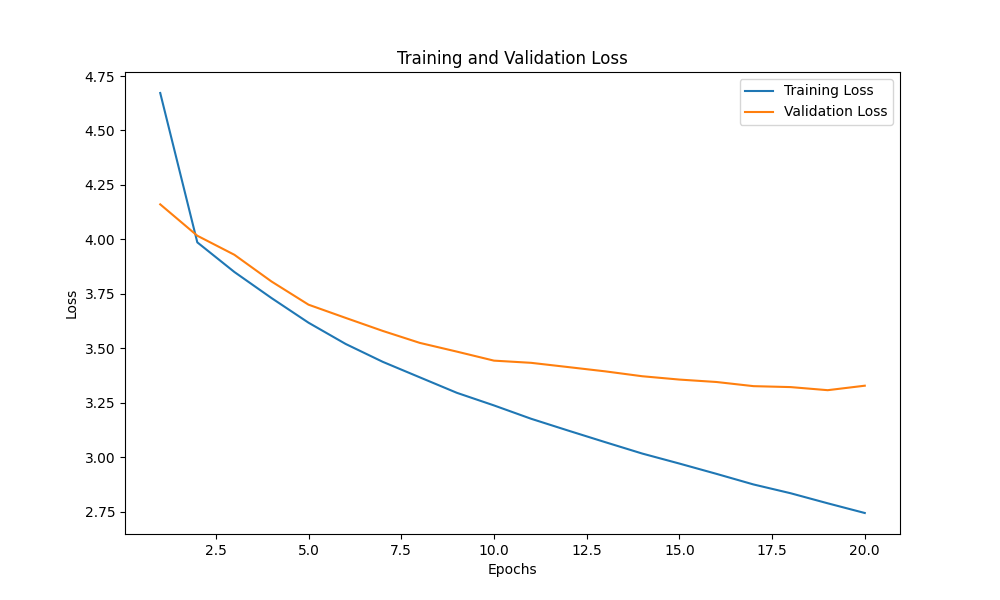
\includegraphics[width=1\textwidth]{loss-plot.png}
    \caption{Loss plot for TransfomerLM (task1)}
    \label{fig:Fig1}
\end{figure}

\section{Task 2}
\subsection{Preprocessing Steps}
The following steps were applied:
\begin{itemize}
    \item \textbf{Lowercase Conversion:} All input text is converted to lowercase to eliminate case-based discrepancies.
    \item \textbf{Contraction Expansion:} Contractions (e.g., ``can't'') are expanded to their full forms (e.g., ``cannot'') using the \texttt{contractions} library.
    \item \textbf{Abbreviation Expansion:} Common abbreviations (e.g., ``gov.'') are replaced with their full forms (e.g., ``governor'') using a predefined dictionary.
    \item \textbf{URL Removal:} URLs are removed using regular expressions to avoid non-informative tokens.
    \item \textbf{Special Character Removal:} Unnecessary special characters are removed while preserving essential punctuation for readability.
    \item \textbf{Whitespace Normalization:} Extra whitespace is removed to standardize the input text.
\end{itemize}

\subsection{Model Architecture and Hyperparameters}
The primary model used in this task is BART.

\subsubsection*{Model Architecture}
\begin{itemize}
    \item \textbf{BART:} An encoder-decoder architecture that efficiently handles tasks like summarization and, in this case, claim normalization.
    \item \textbf{Tokenizer:} The model utilizes the associated BART tokenizer which handles tokenization, padding, and truncation.
\end{itemize}

\subsubsection*{Hyperparameters}
Key hyperparameters include:
\begin{itemize}
    \item Learning Rate: $3\times10^{-5}$
    \item Weight Decay: $0.01$
    \item Warmup Steps: $500$
    \item Maximum Input Length: $512$ tokens
    \item Maximum Target Length: $128$ tokens
    \item Batch Size: $8$ during training (with a larger batch size for inference when memory permits)
    \item Number of Training Epochs: $3$
    \item Beam Search: Beam size of $4$ is used during generation to improve prediction quality.
\end{itemize}

\subsection{Training and Validation Loss Plots}
\begin{figure}[H]
    \centering
    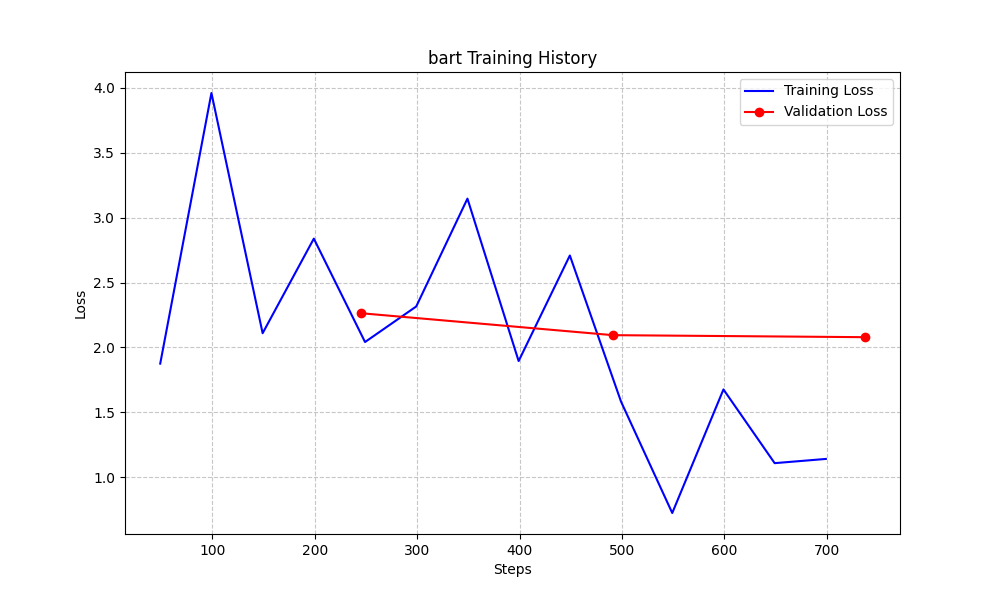
\includegraphics[width=1\textwidth]{bart_loss (1).png}
    \caption{Loss plot for Bart}
    \label{fig:Fig1}
\end{figure}

\begin{figure}[H]
    \centering
    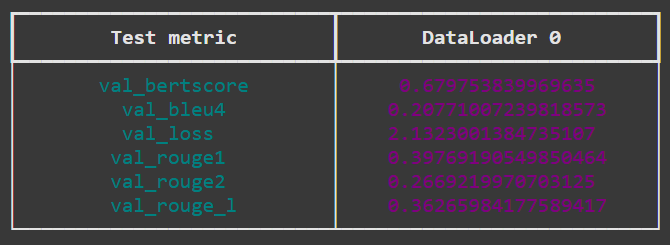
\includegraphics[width=1\textwidth]{bart_metric.png}
    \caption{Bart Metric}
    \label{fig:Fig1}
\end{figure}


\begin{figure}[H]
    \centering
    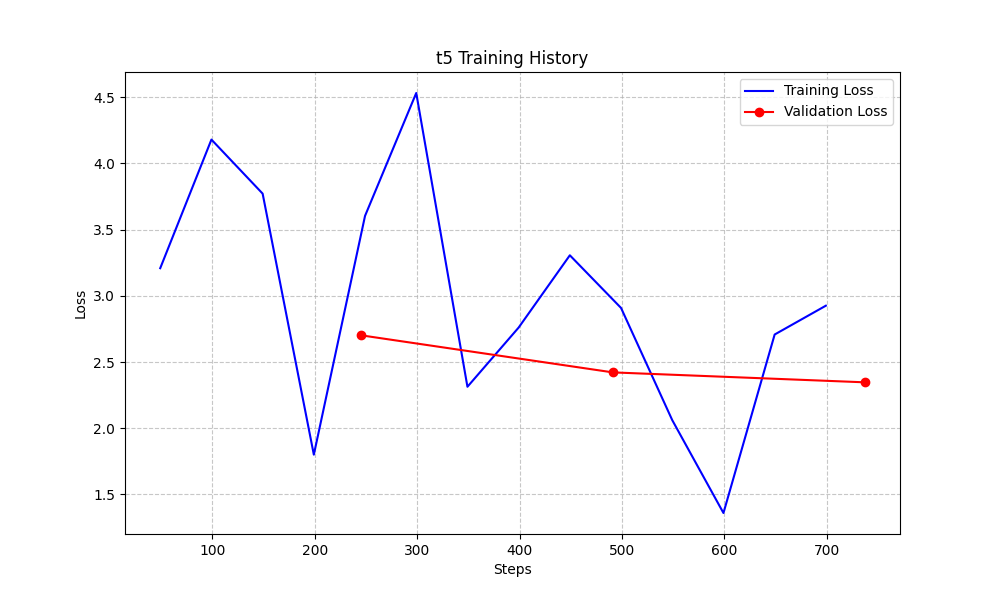
\includegraphics[width=1\textwidth]{t5_loss.png}
    \caption{Loss plot for T5}
    \label{fig:Fig1}
\end{figure}

\begin{figure}[H]
    \centering
    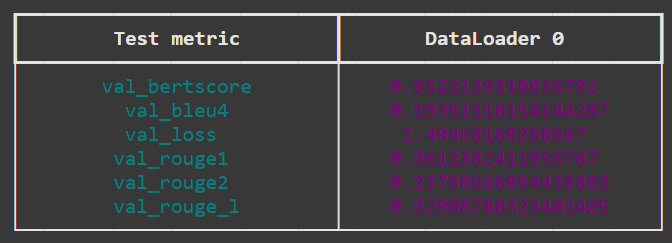
\includegraphics[width=1\textwidth]{t5_metric.png}
    \caption{T5 Metric}
    \label{fig:Fig1}
\end{figure}


\subsection{Evaluation Metrics on the Test Set}

\begin{figure}[H]
    \centering
    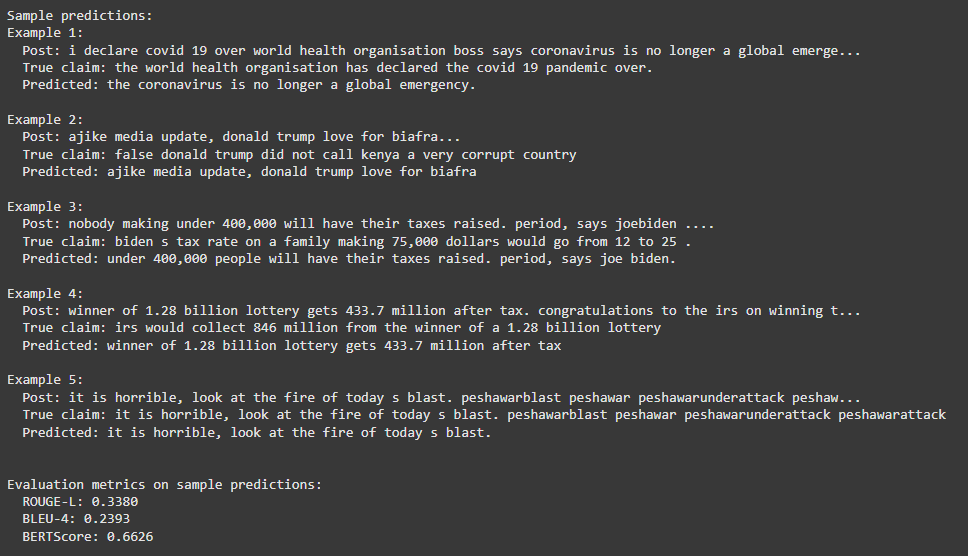
\includegraphics[width=1\textwidth]{bart_predictions.png}
    \caption{Predictions for Samples in Test Dataset using BART}
    \label{fig:Fig1}
\end{figure}
\begin{figure}[H]
    \centering
    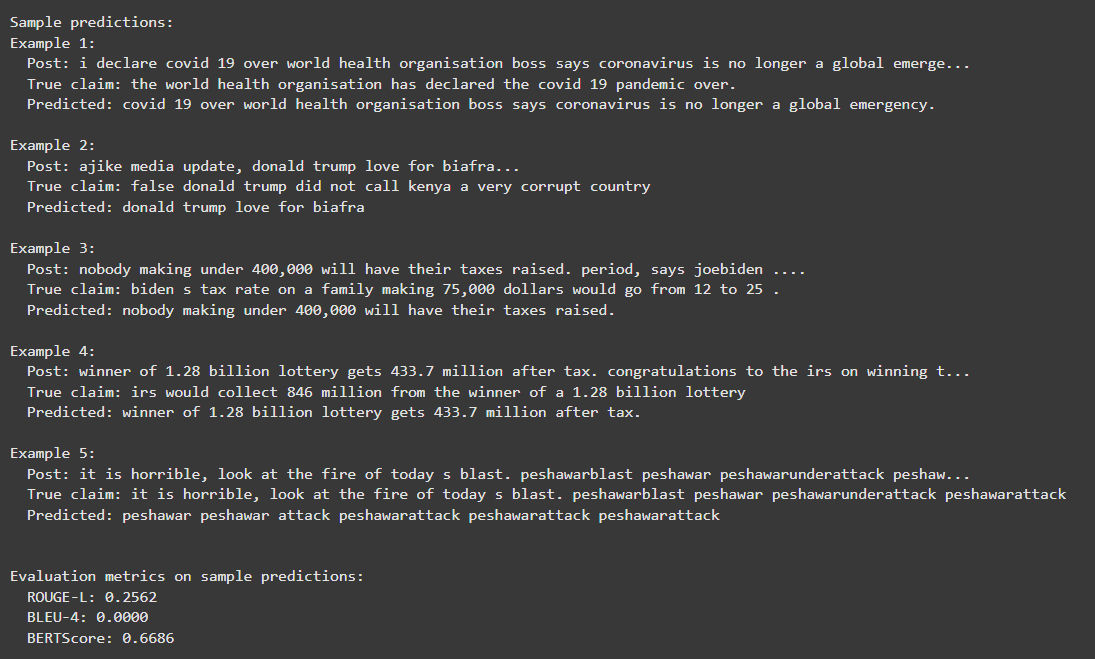
\includegraphics[width=1\textwidth]{t5_predictions.png}
    \caption{Predictions for Samples in Test Dataset using T5}
    \label{fig:Fig1}
\end{figure}
\subsection{Comparative Analysis of Model Performance}
Two models were considered during experimentation:
\begin{itemize}
    \item \textbf{BART:} Achieved strong performance with consistent loss reduction and high evaluation scores on the test set. Its encoder-decoder architecture proved effective for the normalization task.
    \item \textbf{T5:} Preliminary comparisons suggest that while T5 is efficient, the BART model yielded better results under the specific experimental conditions.
\end{itemize}

The comparison is illustrated in the metrics bar chart (\texttt{plots/model\_comparison.png}), which visually contrasts the performance based on ROUGE-L, BLEU-4, and BERTScore.

\subsection{Discussion on Resource Constraints and Model Selection}
Resource constraints played a significant role in the model selection and training process:
\begin{itemize}
    \item \textbf{Hardware Availability:} The experiments were optimized to utilize available GPU resources. When GPUs were not available, the code automatically fell back to CPU execution.
    \item \textbf{Memory Management:} Batch sizes and maximum sequence lengths were carefully chosen to avoid memory overload, ensuring that the training process was both stable and efficient.
    \item \textbf{Computational Efficiency:} BART was preferred due to its balance between performance and computational demands. Although T5 is a robust alternative, its larger model size and higher computational requirements made it less favorable given the available resources.
    \item \textbf{Scalability:} The training and inference pipelines were designed to process data in batches. This approach not only enhanced scalability but also minimized the risk of exhausting computational resources during experimentation.
\end{itemize}

\section{Task 3}
\subsection{Preprocessing}
\begin{itemize}
    \item \textbf{Dataset Loading:} The dataset is loaded from a TSV file containing columns for \texttt{pid}, \texttt{text}, \texttt{explanation}, and \texttt{target\_of\_sarcasm}. Additional image descriptions and detected objects are loaded from pickle files.
    \item \textbf{Text Preprocessing:} For each sample, the text components (\texttt{sarcasm\_target}, \texttt{text}, image description, and detected objects) are concatenated into a single input string.
    \item \textbf{Image Preprocessing:} Images are loaded from a specified directory (with \texttt{.jpg} extension) and transformed using resizing to \(224 \times 224\), conversion to tensor, and normalization (mean = [0.5, 0.5, 0.5] and std = [0.5, 0.5, 0.5]).
    \item \textbf{Tokenization:} The concatenated text inputs and target explanations are tokenized using the \texttt{BartTokenizer}, with padding and truncation applied (maximum length of 256 for inputs and 64 for targets).
    \item \textbf{Custom Collation:} A custom collate function is used to batch the tokenized inputs, targets, and images.
\end{itemize}

\subsection{Model Architecture \& Hyperparameters}
\begin{itemize}
    \item \textbf{Model Components:}
    \begin{itemize}
        \item \textbf{Text Encoder-Decoder:} \texttt{BartForConditionalGeneration} (using the \texttt{facebook/bart-base} checkpoint) is used for generating the explanation text.
        \item \textbf{Image Encoder:} \texttt{ViTModel} (using the \texttt{google/vit-base-patch16-224} checkpoint) extracts image features.
        \item \textbf{Fusion:} A linear fusion layer projects the ViT global image feature to the dimensionality of BART’s hidden states. The projected image feature is added (broadcast) to each token embedding from BART's encoder.
    \end{itemize}
    \item \textbf{Hyperparameters:}
    \begin{itemize}
        \item \textbf{Input and Target Tokenization:} Maximum token length of 256 for input text and 64 for target explanation.
        \item \textbf{Training:} 
            \begin{itemize}
                \item Optimizer: AdamW with a learning rate of \(5 \times 10^{-5}\).
                \item Batch size: 8.
                \item Number of epochs: 3.
            \end{itemize}
        \item \textbf{Generation Settings (Validation):}
            \begin{itemize}
                \item Decoding: Beam search with sampling.
                \item Number of beams: 4.
                \item Maximum generation length: 64 tokens.
                \item Temperature: 1.5.
                \item Top-K: 50.
                \item Repetition penalty: 2.0.
                \item No-repeat n-gram size: 3.
                \item Early stopping enabled.
            \end{itemize}
        \item \textbf{Post-processing:} A custom function is applied to remove repeated sentences and collapse repeated tokens.
    \end{itemize}
\end{itemize}

\subsection{Evaluation}
\textbf{Training Loss and Validation Loss:}\\[5mm]
\begin{tabular}{lcc}
\toprule
\textbf{Epoch} & \textbf{Training Loss} & \textbf{Validation Loss} \\
\midrule
Epoch 1 & 3.1209 & 0.1868 \\
Epoch 2 & 0.1065 & 0.0101 \\
Epoch 3 & 0.0321 & 0.0029 \\
\bottomrule
\end{tabular}

\vspace{5mm}
\textbf{Evaluation Metrics on Validation Set:}\\[5mm]
\begin{tabular}{lccc}
\toprule
\textbf{Metric}    & \textbf{Epoch 1} & \textbf{Epoch 2} & \textbf{Epoch 3} \\
\midrule
ROUGE-1          & 0.0665         & 0.0379         & 0.0375         \\
ROUGE-2          & 0.0003         & 0.0000         & 0.0005         \\
ROUGE-L          & 0.0627         & 0.0369         & 0.0359         \\
BLEU             & 0.0078         & 0.0046         & 0.0046         \\
METEOR           & 0.0411         & 0.0223         & 0.0229         \\
BERTScore\_F1    & 0.7759         & 0.7685         & 0.7611         \\
\bottomrule
\end{tabular}

\vspace{5mm}
\textbf{Sample Generated Explanations (Validation)}\\[3mm]
\begin{itemize}
    \item \textbf{GT:} \textit{the author is pissed at \textless user\textgreater for not getting network in malad.}\\
    \textbf{Pred:} \textit{the the what which that this this this these such so soso so SOSO SO sooooooooooooooooooooooooooooooooooooooo}
    \item \textbf{GT:} \textit{nothing worst than waiting for an hour on the tarmac for a gate to come open in snowy, windy chicago.}\\
    \textbf{Pred:} \textit{the what what what which that this these these these These these such such such a aaaaaaaaaaahaaaaAAAAAABABABABaBaBa Ba Bailey}
    \item \textbf{GT:} \textit{nobody likes getting one hour of their life sucked away.}\\
    \textbf{Pred:} \textit{springspringspringpringspringspring spring springs spring sprang sprung spring rise rises rise rose rise rising rise rise rise risen rise up above below above over above above above lower bottom}
\end{itemize}
\begin{figure}[H]
    \centering
    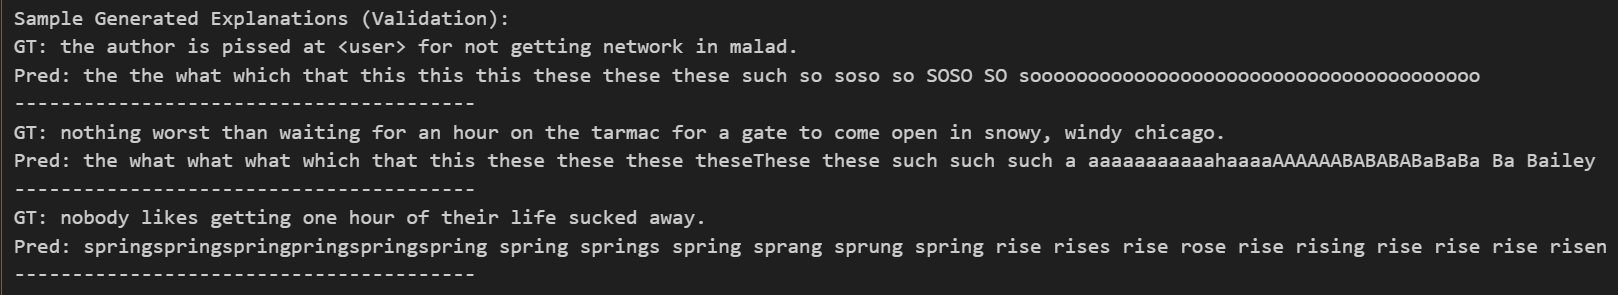
\includegraphics[width=0.8\linewidth]{image.png}
\end{figure}

\section{Individual Contribution}
\begin{itemize}
    \item Himanshu Raj: Task 1 implementation and report
    \item Ishita: Task 2 implementation and report
    \item Ritika Thakur: Task 3 implementation and report
\end{itemize}

\section{References}
\begin{itemize}
    \item \hyperlink{https://drive.google.com/file/d/1mMX4NhoZovPh8pJNbMpmV_EWy43CoBPO/view}{Target-Augmented Shared Fusion-based Multimodal Sarcasm Explanation Generation}
\end{itemize}

\end{document}